

Anteriormente la técnica que se empleaba para poder obtener imágenes de la estructura de los vasos sanguíneos era la angiografía clásica, la cual, requiere de la introducción de un catéter, de una solución de contraste y de rayos X para poder observar los tejidos vasculares. Posterior a la aplicación de la resonancia magnética para la observación de tejidos, se implementó la angio-resonancia o angiografía por resonancia magnética. El objetivo de esta técnica es crear un contraste entre el flujo sanguíneo y el tejido circundante relativamente estático para representar y caracterizar los vasos sanguíneos. Debido a que no utiliza agentes de contraste o rayos X, posee la ventaja de ser un procedimiento de carácter no invasivo e inocuo. En este capítulo tan solo nos referiremos a la obtención de imágenes sensibles a los movimientos macroscópicos de líquidos orgánicos con un flujo resultante neto, como el que produce el flujo sanguíneo, sin entrar a considerar la obtención de imágenes sensibles a los movimientos microscópicos que es en los que se basan las técnicas de difusión. A continuación, se presentarán las técnicas utilizadas en angiografía por resonancia magnética, así como los principios físicos en los cuales versa la generación del contraste sanguíneo, los factores que influyen tanto positiva como negativamente en la formación y calidad de las imágenes y algunas de sus aplicaciones en el ámbito clínico como método diagnóstico.



Como hemos analizado en capítulos anteriores, en el ámbito de las ciencias biomédicas, la resonancia magnética (RM) es utilizada para obtener imágenes estructurales del cuerpo humano cuando éstos, son sometidos a un potente campo electromagnético, gradientes de campo y a secuencias de pulsos de radiofrecuencias (RF), en donde los protones de los átomos de hidrógeno (H) o espines presentan dos fenómenos de manera simultánea; la relajación longitudinal o \Tone y la relajación trasversal o \Ttwo, donde se produce la reemisión de la energía de RF previamente absorbida para generar el eco o señal. La información obtenida de la señal, posteriormente es digitalizada para poder reconstruir la imagen anatómica.

Bajo el entendimiento de esta metodología, es importante destacar que la RM es muy sensible al movimiento de espines contenidos en un medio líquido, siendo el flujo sanguíneo, uno de los de mayor relevancia en la RM. El flujo sanguíneo es considerado como un volumen de sangre que fluye en el interior de un vaso sanguíneo, a través de cualquier tejido, en un determinado periodo de tiempo. El proceso dinámico del flujo sanguíneo es responsable de la generación de fenómenos denominados artefactos de flujo sanguíneo, que hasta cierto punto pueden minimizar el valor diagnóstico de las imágenes obtenidas, por lo que normalmente hay que evitarlos. Sin embargo, podemos tomar ventaja de este artefacto para la obtención de imágenes detalladas de la anatomía vascular sin la utilización de sustancias de contraste, de donde surge la técnica denominada angio-resonancia o angiografía por resonancia magnética. 

La angiografía por resonancia magnética (ARM) es un tipo de imagenología en la que se logran diferenciar los espines de voxeles que presentan un movimiento neto en su interior producido por el flujo sanguíneo, respecto de los espines que se localizan en voxeles sin un movimiento neto, a los que podremos denominar como voxeles ``móviles'' y ``estacionarios'' respectivamente. Esta diferencia de movimiento entre voxeles nos permitirá tomar ventaja, durante la absorción de energía de pulsos de RF o durante la perdida de fase de los espines, para generar el contraste en la imagen. Las técnicas fundamentales utilizadas en ARM son divididas básicamente en relación al contraste que generan respecto al tejido que lo rodea, por lo que se utilizan técnicas de contraste en ``sangre negra'' (hipointensa) y de ``sangre blanca'' (hiperintensa).

\section{ARM con técnicas de contraste en sangre negra}
Las técnicas de sangre negra o Black Blood tienen como objetivo evidenciar el flujo sanguíneo con un contraste más negro respecto al tejido estático circundante. Las secuencias de pulsos utilizadas de forma habitual en la obtención de este tipo de contraste son las Spin Echo (SE) o sus variantes Multi-echo (dual-echo), Turbo Spin Echo o Inversion Recovery (IR). 

Para que un espín produzca señal en secuencias SE, es necesario que reciba tanto el pulso de 90º como el de 180º; en caso contrario no habrá señal. Por lo tanto, cuando en la rebanada de interés hay un vaso sanguíneo que la atraviesa perpendicularmente, al enviar un pulso de RF selectivo a rebanada de 90º que dirija el vector de magnetización al plano transversal, éste no solo excitará a los espines del tejido estático, sino también a los del flujo sanguíneo local que pasa en ese momento por el vaso sanguíneo. Dada la dinámica del flujo, los espines móviles que se han excitado por el primer pulso de RF, se relajan mientras van saliendo de la rebanada en cuestión. Paulatinamente, el flujo sanguíneo previamente excitado será sustituido por sangre nueva que no ha sido excitada, por lo que cuando se emita el segundo pulso selectivo de RF (de 180º) para refasar los espines y obtener la señal, la sangre nueva solo recibirá este segundo pulso, siendo incapaz de poder brindar el eco. Lo que aparecerá en la imagen es un ``vacío de señal'' en el lugar que debía ocupar la sangre, observándose en negro respecto a los demás tejidos estáticos que si recibieron toda la secuencia de pulsos (Figura \ref{fig:arm_image1}). 


\begin{figure}[htb]
\begin{figg}
 \includegraphics[width=\textwidth]{fig_arm_image1}
 \caption{Obtención de imágenes con contraste en sangre negra. A) Secuencia de pulsos SE. B) Se muestra el efecto que presenta la secuencia SE sobre una rebanada por donde cruza perpendicularmente un vaso sanguíneo, se puede observar como todos los espines cambian su vector de magnetización al plano transversal después del pulso de 90º. Después los espines del flujo sanguíneo salen y son reemplazados por espines nuevos totalmente relajados, antes del pulso de refase de 180º el cual tendrá efecto únicamente sobre espines del tejido estático que finalmente serán los que brindarán la señal. C) Imagen axial del ventrículo derecho del corazón obtenida mediante una secuencia Black-Blood o de sangre negra. AD: aurícula derecha; AI: aurícula izquierda; VD: ventrículo derecho; VI: ventrículo izquierdo.}
 \label{fig:arm_image1}
\end{figg}
\end{figure}



Una secuencia utilizada en contraste en sangre negra es la IR doble (DIR), la cual utiliza la aplicación previa de dos pulsos de RF inversores que permiten suprimir la señal de la luz del vaso sanguíneo. Esto se logra aplicando un pulso de inversión no selectivo de 180º precedido por un pulso de inversión selectivo de 180º que devuelve al vector de magnetización sobre el plano longitudinal original, pero sólo de los espines contenidos en la rebanada, para aplicar después nuestra secuencia de pulsos SE y producir la señal. El Tiempo de Inversión (TI: tiempo entre el segundo pulso inversor y el primer pulso excitador) se calcula de manera que los espines de la sangre estén pasando por el punto cero de magnetización longitudinal y no den señal. De esta manera los espines que han recibido el segundo pulso inversor salen del corte y son sustituidos por los espines anulados que provienen de fuera del corte y que paulatinamente van recuperando su vector de magnetización longitudinal y pueden emitir un eco al recibir toda la secuencia de pulsos (Figura \ref{fig:arm_image2}). 



\begin{figure}[htb]
\begin{figg}
 \includegraphics[width=\textwidth]{fig_arm_image2}
 \caption{Secuencia de Pulsos ``Inversion Recovery'' doble (DIR). A) Se ejemplifica la aplicación de dos pulsos de RF inversores, uno no selectivo y otro selectivo a rebanada, con la posterior aplicación de la secuencia SE para recuperar la señal. B) Se muestra el efecto de cada pulso de RF de la secuencia DIR sobre el vector de magnetización hasta la obtención del eco, en relación al marco de referencia de rotación. }
 \label{fig:arm_image2}
\end{figg}
\end{figure}



Cuando el flujo es ortogonal al corte, el efecto de sangre negra aumenta a medida que incrementa la velocidad de la sangre, menor es el grosor del corte y menor es el parámetro TE establecido. La presencia de un flujo lento contenido en el mismo plano que la imagen produce que la sangre se observe brillante, lo que provoca confusión con patologías intravasculares como en el caso de la trombosis, por lo que podríamos aumentar ligeramente el valor del TE respecto al valor de \Tone del tejido para asegurar el contraste. Además, es conveniente hacer la comparación de imágenes con contraste en sangre negra respecto de imágenes con contraste en sangre blanca, para excluir ciertas patologías que pueden estar enmascaradas y que a nivel diagnostico son de relevancia en enfermedades vasculares de inicio. 

Para poder conseguir la máxima velocidad del flujo y aumentar el contraste, un procedimiento clásico es hacer una sincronización cardiaca  entre el TI y la sístole cardiaca con un valor de TR igual al intervalo R-R del electrocardiograma (ECG) (Figura \ref{fig:arm_image3}). Dado que la potenciación de las imágenes depende del valor del TR y TE, cuando el TR es igual al tiempo de un intervalo R-R, el TE tiene que ser corto para poder obtener imágenes potenciadas en \Tone, mientras que cuando el TR es igual a 2 o más intervalos R-R, el TE tiene que ser largo para obtener imágenes potenciadas en \Ttwo. 




\begin{figure}[htbp]
\begin{figg}
 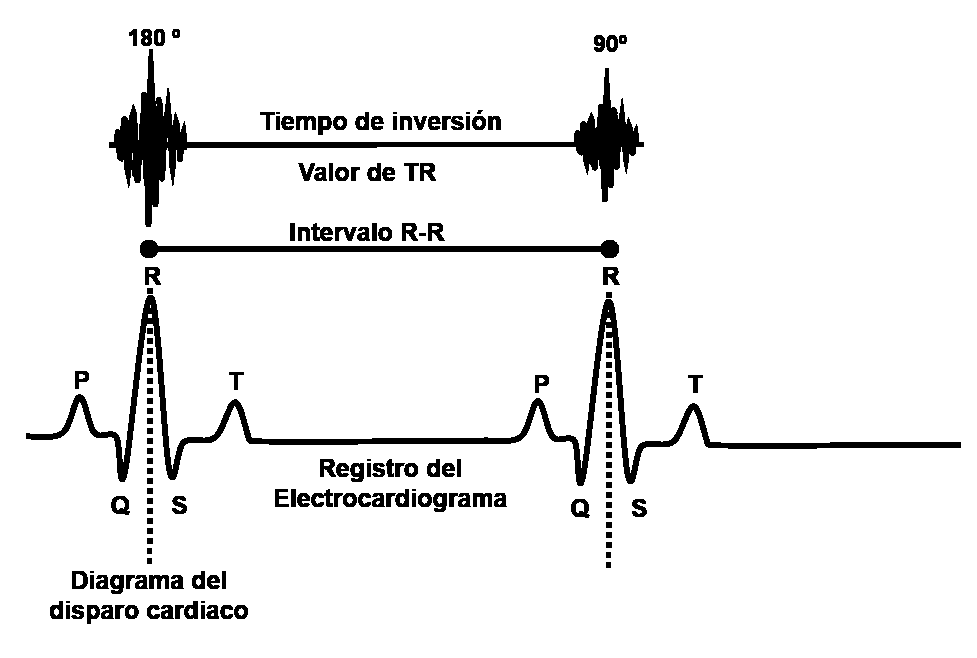
\includegraphics[width=\textwidth]{fig_arm_image3}
 \caption{Secuencias de sincronización.  Se muestra la sincronización cardiaca del intervalo R-R del ECG con el Tiempo de inversión (tiempo entre los pulsos de 180º y 90º). }
 \label{fig:arm_image3}
\end{figg}
\end{figure}


Una de las principales aplicaciones de la ARM en contraste con sangre negra es en área de la cardirresonancia debido a que las imágenes generadas, fundamentalmente se utilizan para obtener información anatómica del corazón.

\section{ARM con Técnicas de sangre blanca}
La ARM con contraste en sangre blanca o Bright Blood permite que el flujo sanguíneo aparezca más brillante que los tejidos estáticos. Se utilizan básicamente dos técnicas denominadas tiempo de vuelo o ``Time-Of-Flight'' (TOF) y las técnicas con contraste de fase o ``Phase Contrast'' (PC). 


\subsection{Técnica de ARM ``Time-Of-Flight''  (TOF) }

La ARM con efecto TOF se fundamenta en cambios en la magnetización longitudinal o \Tone. La primera observación del efecto TOF fue realizada por Suryan en 1951, quien observó que el valor del \Tone del agua en movimiento era más corto que el valor del \Tone del agua estacionaria. Estableciendo que esta diferencia era atribuida al hecho de que en estado estacionario, los espines pueden ser saturados con pulsos de RF, pero cuando están en movimiento, espines ``frescos'' podían reemplazar la magnetización de los espines estacionarios, por lo que incrementaban su señal. 

La ARM con efecto TOF se lleva a cabo utilizando secuencias Echo de Gradientes (EG). En este caso se realiza la aplicación repetitiva de pulsos de RF no selectivos que provocan la saturación del vector de magnetización, principalmente del tejido estático. Posteriormente, cuando se aplique el pulso de RF selectivo de 90º, solo producirá señal el flujo sanguíneo en movimiento debido a que su vector de magnetización longitudinal no está saturado. En esta técnica para poder saturar el tejido estacionario se utilizan valores de TR menores que su valor de \Tone y valores de TE cortos para lograr la obtención de la señal durante la emisión del eco en el TOF del plano (Figura \ref{fig:arm_image4}). 


\begin{figure}[htbp]
\begin{figg}
 \includegraphics[width=\textwidth]{fig_arm_image4}
 \caption{
 Saturación del tejido estático con pulsos de RF repetitivos. A) Se muestra la aplicación de pulsos de RF repetitivos no selectivos que paulatinamente saturan el vector de magnetización de los espines de voxeles estacionarios, mientras que los espines de voxeles móviles pueden recuperar su vector de magnetización tras cada pulso de RF por lo que no se saturan. B) Se ejemplifica el mantenimiento y saturación del vector de magnetización de espines móviles y estacionarios respectivamente, en relación al marco de referencia de rotación. 
 }
 \label{fig:arm_image4}
\end{figg}
\end{figure}




La saturación del tejido con la emisión repetida de pulsos de RF no selectivos después de cada TR, provoca que el valor de la magnetización residual vaya disminuyendo paulatinamente hasta alcanzar un estado estacionario (steady state), el cual, será considerado como el valor de magnetización que presentarán los espines de voxeles estacionarios. Mientras que en los voxeles donde continuamente fluye sangre fresca totalmente relajada, el valor del vector de magnetización será mayor, provocando una diferencia de señal proporcional a las diferencias en la magnetización longitudinal entre espines de voxeles estacionarios (saturados) y espines de voxeles móviles (relajados) que sirve para visualizar la luz de los vasos sanguíneos.



Para poder crear la diferencia de señal, el valor de nuestro TR se debe de ir acortando de forma consecutiva tras cada pulso de RF, sin dar tiempo a que los espines de los voxeles estacionarios se relajen por completo. De esta forma el nuevo pulso de RF actuará sobre una magnetización parcialmente saturada evidentemente menor que su valor completo. Mientras que en los voxeles móviles, el nuevo pulso volcará el vector de magnetización con mayor valor, creándose la diferencia de señal. El valor de la señal obtenida es proporcional al número de espines que están ingresando al plano de interés durante cada TR (Figura \ref{fig:arm_image5}). 


\begin{figure}[htbp]
\begin{figg}
 \includegraphics[width=\textwidth]{fig_arm_image5}
 \caption{
Acortamiento del valor del TR para la generación de imágenes con efecto TOF. A) A medida que el valor TR va disminuyendo con valores menores que el valor del \Tone, los espines estacionarios dentro de la rebanada son parcialmente saturado y, por lo tanto, producirán sólo un poco de señal, mientras que los espines en movimiento no se saturan, lo que resulta en una alta intensidad de señal, creando la diferencia de señal. B) Efecto TOF sobre el tejido con secuencias EG. 1) Cuando la sangre es estacionaria se satura al igual que otros tejidos con \Tone largos. 3) A velocidades máximas, cuando $V \geq S/TR$, el máximo flujo sanguíneo de entrada no se satura y se observa una máxima señal. 2) A velocidades intermedias del flujo sanguíneo,$V=S/(2TR)$ habrá un incremento en la señal en comparación con 1) pero menor que 3) debido a la parcial saturación de los espines durante cada TR que se muestra en A).
 }
 \label{fig:arm_image5}
\end{figg}
\end{figure}

Una ventaja de utilizar las secuencias EG es que el eco se obtiene por inversión de gradiente y por lo tanto no es selectivo del plano de interés. Por lo tanto, aunque la sangre salga del plano inicial podremos seguirla y obtener la señal que produzca en otros planos subsecuentes, siempre y cuando se conserve la diferencia de magnetización entre voxeles móviles y estacionario. Las principales limitaciones de esta técnica son el denominado flujo turbulento lo que provoca desfases intravóxel y los vasos sanguíneos que se encuentren muy próximos a tejidos con \Tone cortos, como la grasa o donde haya ocurrido una hemorragia subaguda ya que habrá productos de degradación de la sangre tales como la metahemoglobina que producirán una señal brillante similar al flujo sanguíneo. 

Para la ARM con efecto TOF, el procesado de las imágenes se realiza mediante reconstrucción con un algoritmo de trazado de rayos, llamado máxima intensidad de proyección (MIP: maximum intensity projection), donde el conjunto de datos 3D muestra los vasos desde múltiples puntos de vista en ángulos de 180º alrededor de un eje perpendicular al plano de adquisición original, es decir, sobre una dirección se elige el voxel de máxima intensidad de señal y se proyecta sobre un plano perpendicular, se obtienen entonces imágenes 2D en las que tan solo se representan los valores máximos (Figura \ref{fig:arm_image6}).


\begin{figure}[htbp]
\begin{figg}
 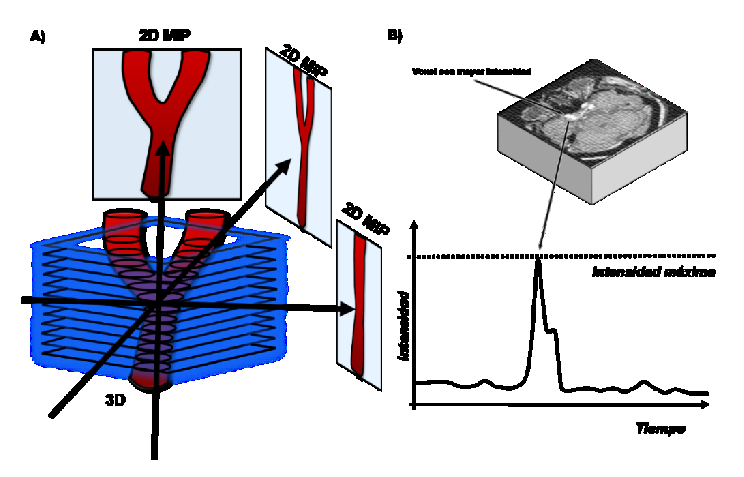
\includegraphics[width=\textwidth]{fig_arm_image6}
 \caption{
Reconstrucción de máxima intensidad de proyección (MIP). Esquema de la obtención de imágenes mediante la técnica MIP. A) Una estructura tridimensional se plasma en un plano, a lo largo de cada rayo de proyección se generan imágenes en 2D, B) sólo el píxeles con la señal de máxima intensidad se proyectan sobre el plano de la imagen. 
 }
 \label{fig:arm_image6}
\end{figg}
\end{figure}



En la técnica MIP no se proyecta la suma de las intensidades recogidas a lo largo del eje de proyección sino tan solo el máximo de sus valores sin tomar en cuenta la intensidad de los otros voxeles. Variando la dirección de proyección se pueden reconstruir, con secuencias CINE, imágenes dinámicas, donde estén los vasos sanguíneos girando tridimensionalmente en el espacio y elegir la mejor proyección para el diagnóstico. 
La técnica TOF puede ser realizada ya sea mediante adquisiciones múltiples de cortes en 2D, así como con adquisiciones volumétricas en 3D, dependiendo principalmente de la resolución espacial necesaria y de la longitud de la zona vascular a explorar. 

\subsection{ARM con técnicas TOF-2D}
En la técnica TOF-2D se realiza la adquisición de cortes delgados en 2D con un grosor de entre 1 a 3 mm, obtenidos de forma adyacente o de manera superpuesta. Una vez obtenida la imagen del primer plano, este es ligeramente desplazado, repitiéndose la adquisición sucesivamente a lo largo de todo el vaso sanguíneo. Adquirir los planos paralelamente uno a continuación del otro le da el nombre de ARM secuencial (Figura \ref{fig:arm_image7}). Posteriormente las imágenes se apilan para formar un conjunto de todos los planos (volumen), la cual se reconstruye por técnicas de proyección o colapso. La obtención de la imagen se hace de forma que el plano sea perpendicular a la dirección del vaso sanguíneo para maximizar el efecto de realce del flujo de entrada. La imagen de colapso es más útil para la visualización de conjuntos de volumen delgado a través del denominado polígono de Willis y para seleccionar regiones de interés de reconstrucciones de imágenes segmentadas. La resolución final depende del grosor elegido para cada corte y este viene condicionado por el valor de los gradientes magnéticos aplicados. 


\begin{figure}[htbp]
\begin{figg}
 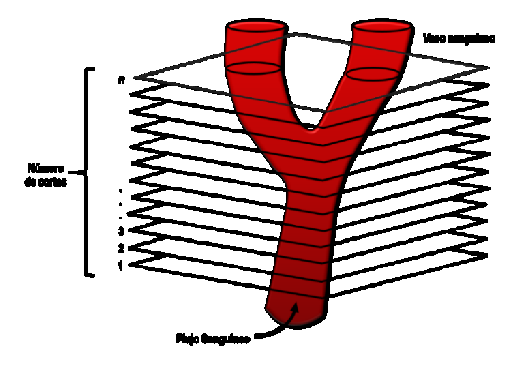
\includegraphics[width=\textwidth]{fig_arm_image7}
 \caption{
Técnica ARM con efecto TOF 2D. Se esquematiza la técnica TOF 2D, la cual se basa en la adquisición de múltiples cortes finos a lo largo de un vaso sanguíneo. El número de cortes adquiridos depende del tamaño del vaso y del espesor de corte. 
 }
 \label{fig:arm_image7}
\end{figg}
\end{figure}



Como el efecto TOF se presenta sobre cualquier vaso que ingrese en el plano de la imagen, independientemente de su dirección, el incremento de señal aparece tanto en las arterias como en las venas aunque tengan sentidos contrarios. Por lo tanto la señal del flujo sanguíneo se puede observar en ambas direcciones en el plano de la imagen. Para poder quitar la señal de los vasos sanguíneos en los que el flujo circula en dirección opuesta al plano de la imagen deseada, se utilizan bandas de pre-saturación adyacentes al plano y del lado de la circulación cuya señal queremos anular, antes de que el flujo sanguíneo entre en el plano de interés y se pueda trasladar con el plano de la imagen. La posición más efectiva de colocar estas bandas de pre-saturación es justo antes de que la sangre (arterial o venosa) entre en el plano de interés y trasladarla con el plano de la imagen, esta forma de obtención de la imagen se llama Walking SAT o Traveling SAT. 
Previo a la obtención de la imagen, estas bandas de pre-saturación son excitadas con un pulso de RF selectivo que provoca que los espines móviles estén en la misma situación que los estacionarios cuando ingresen al plano de interés, de esta forma no generan contraste y se anula la señal del vaso sanguíneo. En la imagen que obtenemos solo queda la señal en la dirección que no está pre-saturada con las bandas (Figura \ref{fig:arm_image8}). 


\begin{figure}[htbp]
\begin{figg}
 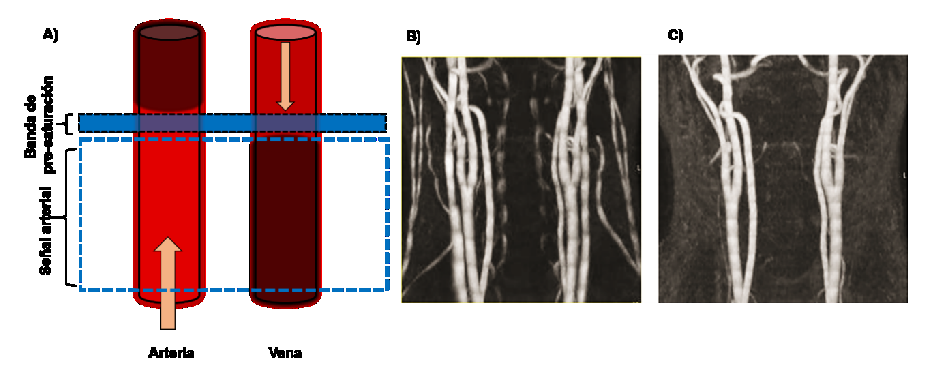
\includegraphics[width=\textwidth]{fig_arm_image8}
 \caption{
Aplicación de bandas de pre-saturación para suprimir la señal del flujo sanguíneo. En A) se esquematiza la colocación de las bandas de pre-saturación para suprimir la señal del flujo sanguíneo venoso. B) Imagen con adquisición sin banda pre-saturación (presencia de flujo venoso y arterial). C) Imagen obtenida con aplicación de banda de pre-saturación; la saturación del flujo venoso permitiendo la visualización solo del flujo arterial. 
 }
 \label{fig:arm_image8}
\end{figg}
\end{figure}



Sin embargo, la TOF 2D resulta ser sensible a los flujos lentos. Esto se debe a que durante la adquisición se usan divisiones muy finas en las que la sangre no se satura tan rápido como en un volumen grande ya que el umbral de velocidad para el completo reemplazo de espines es bajo, y muestran una alta intensidad de señal ya que la sangre tiene que recorrer muy poco espacio dentro del plano durante el TR para generar contraste. La técnica TOF 2D se aplica principalmente en zonas extensas de tejido por la rápida localización vascular para obtener imágenes de flujo estacionario como en venas y arterias carótidas en cuello y extremidades inferiores donde se pueden presentar enfermedades oclusivas que obliteran la pulsación arterial. 

\subsection{ARM con efecto TOF-3D}
En la técnica TOF 3D se realiza la adquisición de todo un volumen de datos (slab), donde una capa de tejido relativamente gruesa de aproximadamente 3-8 cm es excitada con pulsos de RF. Los pulsos excitan todo el volumen de adquisición, con lo que el flujo recibe tantos pulsos como cortes se hayan programado y se satura. Posteriormente, de este volumen se individualizan 32 o 64 divisiones planas o particiones a través de un segundo proceso de codificación de fase en la dirección de la selección del corte (Figura \ref{fig:arm_image9}). La ventaja de la TOF-3D es que las particiones pueden ser de menos de 1 mm de grosor, (entre 0.6 o 0.7 mm), con lo que se logran mejores resoluciones espaciales y visualizaciones del vaso sanguíneo por reducción de efectos de volumen parcial. Además, se incrementa el valor de la relación señal-ruido en imágenes individuales, pero este evento también se produce en el tejido de fondo lo que limita el contraste y la visibilidad de algunos pequeños vasos en el MIP final. 

\begin{figure}[htbp]
\begin{figg}
 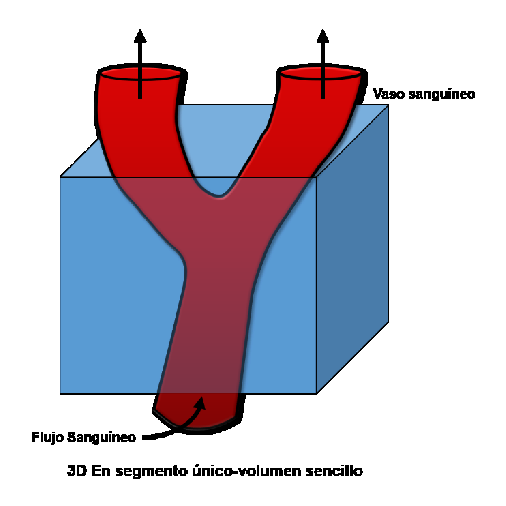
\includegraphics[width=\textwidth]{fig_arm_image9}
 \caption{
Técnica ARM con efecto TOF 3D. En ésta técnica se excita todo el volumen (Slab) al mismo tiempo. La resolución espacial a lo largo de la dirección del slab es similar a la resolución en el plano con una codificación de fase apropiada. 
 }
 \label{fig:arm_image9}
\end{figg}
\end{figure}




Ahora bien, si dentro de nuestro volumen existe un buen contraste del flujo sanguíneo en las zonas iniciales, a medida que este va circulando, la señal va desapareciendo, siendo difícil ver las porciones más distales de los vasos. Igualmente, si la sangre no fluye suficientemente rápido dentro de un volumen delgado de tejido se satura por la excitación repetida, ya que los espines experimentan más pulsos de RF antes de atravesar todo el volumen y se pierde el contraste con respecto a los voxeles estacionarios. 
Existen dos secuencias utilizadas para reducir el efecto de la saturación de flujo sanguíneo. La primera es una técnica hibrido que combina la mejor resolución espacial de las técnicas TOF-3D con la mejor sensibilidad a los flujos lentos de las técnicas TOF-2D y se denomina Multiple Overlapping Thin Slab Acquisition (MOTSA) o multichunk. Este método tiene como objetivo reducir el efecto de saturación mediante la reducción del grosor de las particiones, pero manteniendo el volumen total. Consiste en partir el volumen total en varios subvolúmenes ligeramente sobrepuestos, de manera que el flujo que recorre cada subvolumen recibe menos pulsos de RF. No obstante, al ensamblar todos los subvolúmenes para obtener la imagen final, se puede presentar un artefacto entre los slab denominado ``persiana veneciana'' (Venetian Blind), donde el tejido de fondo tiende a ser más brillante en la parte de arriba de cada slab debido al incremento del ángulo de inclinación. Cuando se empalman los slabs existe diferencia de señal del tejido de fondo entre la parte de abajo del slab con la parte superior del siguiente slab, lo cual se puede corregir después de reconstruir la imagen (Figura \ref{fig:arm_image10}). 


\begin{figure}[htbp]
\begin{figg}
 \includegraphics[width=\textwidth]{fig_arm_image10}
 \caption{
Secuencia Multiple Overlapping Thin Slab Acquisition (MOTSA). En A) se representa la técnica MOTSA que se basa en la adquisición de múltiples slabs finos 3D secuenciales y ligeramente superpuestos donde el área gris representa el solapamiento. B) Se muestra el artefacto de persiana veneciana en los límites entre slabs.
 }
 \label{fig:arm_image10}
\end{figg}
\end{figure}



La segunda secuencia utilizada para mejorar el efecto de saturación sanguínea es la denominada Tilted Optimized Non-saturating Excitation (TONE), en la cual se genera una variación en el ángulo de inclinación de los pulsos de RF de manera lineal a lo largo de todo el volumen de adquisición 3D, tomando valores más pequeños al principio del slab y aumentando su valor paulatinamente con respecto al tiempo hasta el final del slab, para asegurar que los espines no sean saturado demasiado rápido (Figura \ref{fig:arm_image11}).


\begin{figure}[htbp]
\begin{figg}
 \includegraphics[width=\textwidth]{fig_arm_image11}
 \caption{
Tilted Optimized Non-saturating Excitation (TONE). En A) se muestra el slab con un ángulo de inclinación (XX) contante a lo largo de todo el volumen de la imagen. En B) se esquematiza la variación del ángulo de inclinación de forma creciente a los largo de todo el volumen de adquisición. 
 }
 \label{fig:arm_image11}
\end{figg}
\end{figure}



Finalmente, también la supresión del tejido estático mejora si se utilizan prepulsos de transferencia de magnetización. La trasferencia de magnetización se refiere a un proceso en el cual espines asociados con moléculas de agua de hidratación (no unida o libre), pueden intercambiar sus energías con otros espines de moléculas de agua unidos a macromoléculas que tienen valores de relajación T2 muy cortos y por lo tanto resonancias muy amplias, por lo que son relativamente invisibles a la RM convencional. Para aplicar trasferencia de magnetización pulsos de RF (off-resonance) son utilizados para saturar la magnetización de los espines unidos. Cuando estos espines intercambian su magnetización con los espines libres, hay una importante reducción en la señal que produce el tejido, mientras que la señal del flujo sanguíneo no presenta un efecto de trasferencia de magnetización, por lo que no se ve afectado. El resultado total es un mejor contraste de los vasos sanguíneos con respecto al tejido de fondo (Figura \ref{fig:arm_image12}).



\begin{figure}[htbp]
\begin{figg}
 \includegraphics[width=\textwidth]{fig_arm_image12}
 \caption{
Principio de Trasferencia de magnetización. El efecto de trasferencia de magnetización es empleado para mejorar el contraste del tejido de fondo en imágenes TOF-3D. La aplicación de pulsos de RF provoca que los espines unidos a agua libre intercambien su magnetización con espines de agua unida a macromoléculas provocando un acortamiento en sus valores T2, resultando en un incremento de la señal del tejido de fondo que mejora la visualización de vasos sanguíneos.
 }
 \label{fig:arm_image12}
\end{figg}
\end{figure}




\section{ARM con técnicas de Contraste de Fase (PC)}
La PC se basa en los cambios de fase en la magnetización trasversal o T2, entre los espines de la sangre con respecto a los del tejido estacionarios a lo largo del gradiente. La técnica con PC es una secuencia EG en la que se aplica un gradiente bipolar de igual duración e intensidad pero con signos contrarios para codificar la velocidad de flujo, el cual provoca un desfase que dependerá de la velocidad de los componentes del tejido.

Cuando se habla de la aplicación de un gradiente bipolar en un sistema se refiere uno a lo siguiente: Si dentro de una rebanada de interés se encuentran dos grupos de espines, ubicados en un punto A y un punto B, separados por una cierta distancia y son sometidos a un gradiente de campo (Gradiente de desfase: +GZ), en dirección de A a B, ambos grupos de espines estarán sometidos a campos magnéticos distintos donde los espines ubicados en el punto B perciben un campo magnético mayor que los espines en el punto A, modificando sus frecuencias de precesión. Al emitir un pulso de RF se provoca que los espines de ambos grupos entren en resonancia. En el tiempo cero ($t_0$) sus proyecciones sobre el plano trasversal estarán orientadas de la misma forma, es decir, estarán en fase. Sin embargo, conforme avanza el tiempo los espines en B se adelantan respecto a los espines en A dadas las diferencias en sus frecuencias de precesión. Al ángulo formado por las diferentes posiciones entre espines en el $t_0$ se denominará como $\phi$. 

Conforme avanza el tiempo, phi se va incrementando debido al desfase entre espines, siendo mayor $\phi_A$ que $\phi_B$, formando un ángulo de desfase entre espines directamente proporcional al tiempo trascurrido. Si después de cierto tiempo se apaga el gradiente de campo y se aplica un segundo gradiente de la misma magnitud que el primero durante el mismo tiempo, pero de sentido contrario, es decir de B a A (Gradiente de refase: -GZ) el efecto sobre el sistema será invertido. Los espines en A precesarán a mayor frecuencia que los de B, de esta manera se induce que los espines vuelven a estar en fase. El par de gradientes (+Gz y -Gz) aplicados es lo que constituye al gradiente bipolar (Figura \ref{fig:arm_image13}). 


\begin{figure}[htbp]
\begin{figg}
 \includegraphics[width=.75\textwidth]{fig_arm_image13}
 \caption{
Fenómeno físico de la técnica de Contraste de Fase sobre espines estáticos. A) Dos grupos de espines son sometidos a un gradiente de campo +Gz dirigido de A a B. La aplicación de un pulso de RF produce que los espines entren en resonancia. B) Sus proyecciones sobre el plano transversal quedan orientadas de la misma forma (en fase). C) Debido a la diferencia en las frecuencias de precesión, el ángulo $\phi_B$ es mayor que el ángulo $\phi_A$. D) La aplicación de un gradiente –Gz invierte el sistema y refasa los espines. E) La aplicación del gradiente bipolar satura los espines puesto que primero se desfasan un cierto ángulo en un sentido y después el mismo ángulo en sentido contrario lo que permite codificar el flujo. 
 }
 \label{fig:arm_image13}
\end{figg}
\end{figure}



Ahora bien, se dentro de nuestro sistema existen espines móviles que pueden estarse desplazando del punto A al B, como los del flujo sanguíneo, al momento de cambiar el valor del campo magnético que perciben a lo largo de su trayectoria, al aplicarles el segundo gradiente, estos espines no logran refasarse con los espines estacionarios cuando lleguen al punto B, y por lo tanto acumulan fase. Este fenómeno se denomina como desfase de flujo ($\phi_f$) y es directamente proporcional a la velocidad a la que se mueven los espines a lo largo del gradiente (Figura \ref{fig:arm_image14}). No obstante, el desfase de flujo no solo depende de la velocidad del mismo, sino también de la naturaleza de los gradientes, es decir, del valor, la forma y el tiempo de aplicación del gradiente bipolar, denominado como primer momento del gradiente (M). Formalmente se representa de con la siguiente formula:

\begin{equation}
 \phi_f = \gamma\nu * M * t
\end{equation}

donde $\gamma$ es la constante giromagnética del protón de H, $\nu$ la velocidad en dirección al gradiente bipolar aplicado, $t$ el intervalo de tiempo entre los dos gradientes y $M$ el área de cada uno de los dos  gradientes.



\begin{figure}[htbp]
\begin{figg}
 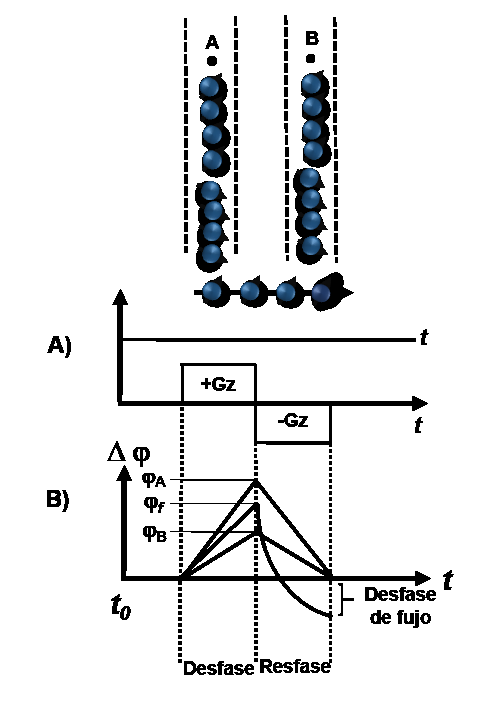
\includegraphics[width=.75\textwidth]{fig_arm_image14}
 \caption{
 Efecto del gradiente bipolar sobre espines móviles. A) Si espines móviles se desplazan bajo el gradiente bipolar no se saturan y B) acumula un desfase ($\phi_f$) respecto a los núcleos estacionarios, ya que no perciben la misma intensidad de gradiente en un lado que en el otro, puesto que cambian de posición. Este desfase de flujo nos permitirá cuantificar la velocidad del flujo
 }
 \label{fig:arm_image14}
\end{figg}
\end{figure}




Para formar la imagen PC es necesario realizar la adquisición de dos conjuntos de datos sobre la misma dirección pero con diferente sensibilidad al flujo, con el objetivo de evitar cambios de fase no uniformes en los espines. El primer conjunto de datos S1, se adquiere con una secuencia con compensación de flujo que permite definir la fase en la magnetización trasversal. El segundo conjunto de datos, S2, es adquirido con una secuencia sensible al flujo lo que permite codificarlo. Ambas adquisiciones se sustraen automáticamente para eliminar desfases introducidos por causas externas a la técnica. La cantidad de sensibilidad de flujo es controlada por la fuerza del gradiente bipolar incorporado dentro de la secuencia de adquisición. 
Para poder generar las imágenes de fase, una vez finalizadas las dos adquisiciones, se realiza una resta compleja de los valores entre S1 y S2 que se denomina como $\Delta{S}$ y que depende del cambio de fase de $\phi_f$ dentro de cada voxel, donde $\Delta{S}$ obtiene un valor máximo cuando existen direcciones opuestas entre S1 y S2. Por lo tanto, el flujo en dirección contraria al gradiente de codificación no da señal y aparece obscuro, debido al desplazamiento de fase que se presenta dentro de cada voxel (Figura \ref{fig:arm_image15}). La información se presenta en dos tipos de imágenes: la imagen de magnitud y la imagen de fase. En la imagen de fase, la velocidad del espín en cada punto dentro del campo de visión se muestra por la intensidad de la señal de $\Delta{S}$, por lo tanto, los píxeles más brillantes corresponden a las velocidades más altas. 



\begin{figure}[htbp]
\begin{figg}
 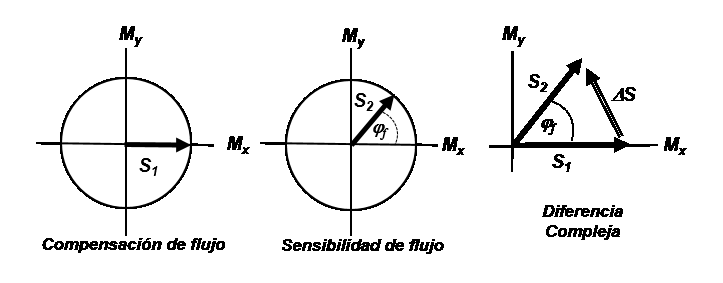
\includegraphics[width=\textwidth]{fig_arm_image15}
 \caption{
Adquisición de las dos conjuntos de datos en la ARM PC. La resta compleja de dos conjuntos de datos que son adquiridos con diferentes sensibilidades al flujo, S1 con compensación de flujo y S2 con sensibilización al flujo producen una imagen con intensidades de señal en función de las velocidades de flujo locales.
 }
 \label{fig:arm_image15}
\end{figg}
\end{figure}



La relación lineal entre la velocidad y el ángulo de fase generada por el gradiente bipolar es ajustado por un conjunto de datos denominado Velocity encoding (VENC) que determina la velocidad máxima a la cual la secuencia podrá codificar adecuadamente la velocidad del flujo sanguíneo de interés sin que exista el artefacto de enrollamiento o \textit{aliasing}. Además, dependiendo de la velocidad del flujo estimada dentro del vaso en estudio, también se definirán los parámetros de las secuencias de adquisición como por ejemplo la amplitud de los pulsos de RF y la amplitud de los gradientes que son utilizados para codificar el flujo. Una limitación de la imagen PC es la necesidad de saber a priori qué velocidad de flujo se espera en el vaso de interés. Gracias a los valores de desfase que se obtiene se pueden generar imágenes angiográficas en 2D y en 3D. 

\subsection{ARM con CF 2D}
La ARM con PC 2D es una técnica en la que se obtiene una sola rebanada delgada de cualquier espesor. La aplicación del gradiente bipolar se realiza a lo largo de la dirección de corte, con lo que se codifican velocidades de flujo perpendiculares al mismo y se produce la cancelación de la señal de regiones donde los vasos sanguíneos tienen un flujo en dirección opuesta que se sobrepone a la dirección de la proyección. La obtención de rebanadas delgadas, requiere de dos ligeras modificaciones en la técnica. Primero, debido a que los vasos sanguíneos no solo ocupan una pequeña proporción del volumen de la rebanada, un gradiente de desfase adicional es aplicado en la dirección de la rebanada seleccionada. Esto tiene como objetivo reducir el tamaño de la señal proveniente de tejido estacionario. Y segundo, se debe realiza la resta compleja entre los vector de magnetización la cual produce una mejor calidad en la imagen (Figura \ref{fig:arm_image16}). 


\begin{figure}[htbp]
\begin{figg}
 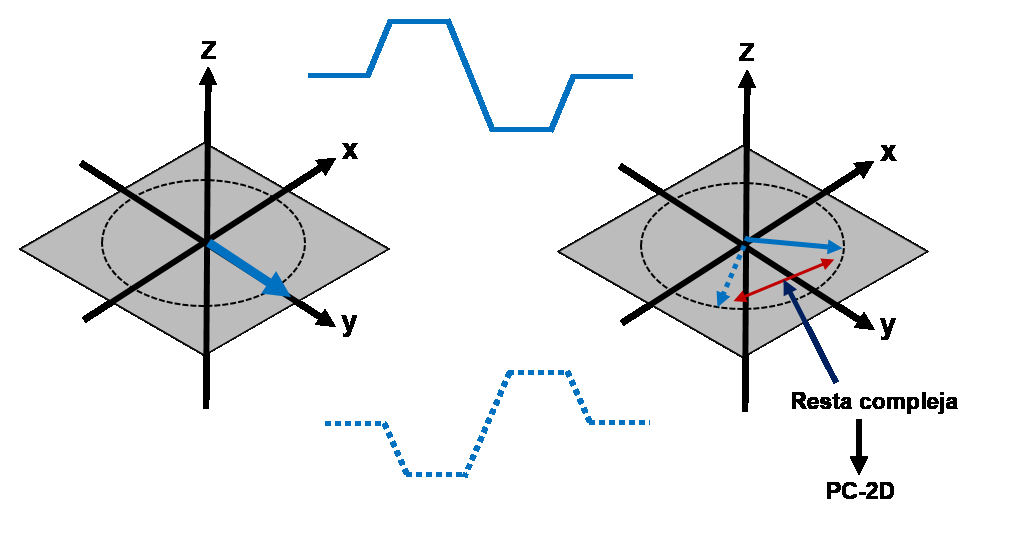
\includegraphics[width=\textwidth]{fig_arm_image16}
 \caption{
Método de procesamiento en ARM PC-2D. Para obtener la imagen se realiza una resta compleja donde se resta el valor del vector de magnetización y que permite generar proyecciones de cortes gruesos con PC-2D.
 }
 \label{fig:arm_image16}
\end{figg}
\end{figure}


 

Debido a que la ARM PC-2D es una técnica en la que se obtiene una única rebanada, las imágenes se pueden obtener con bastante rapidez. De forma alternativa la secuencia se puede combinar con el gatilleo cardiaco, PC-CINE y obtener imágenes cardiacas multifase con resolución temporal para producir imágenes angiográficas con movimiento. Para ello se debe variar el VENC durante el ciclo cardíaco, de manera que haya un VENC corto en la diástole y una grande en la sístole, además la técnica permite adquirir imágenes de flujo tanto lento como rápido. 

\subsection{ARM con CF 3D }
La ARM con PC 3D, es una técnica volumétrica de corte delgado y se aplican gradientes bipolares en las tres direcciones del espacio donde cada corte tiene sensibilización a la velocidad en la dirección requerida. Esto significa que los estudios de PC 3D consumen bastante tiempo y usualmente se debe de sacrificar un poco de resolución en la dirección de la codificación de la fase para reducir los tiempos de análisis. La imagen de velocidad de cada rebanada 3D es procesada con el algoritmo MIP con el fin de generar la imagen. El uso de un bajo VENC significa que se pueden obtener buenas imágenes de flujo lento en 3D. Una de las desventajas de la PC 3D es que necesita de todo el gradiente de codificación de fase, lo que incrementa el valor del TE resultando en una pobre calidad de la imagen en áreas donde el flujo es complejo. En esta técnica se debe aplicar una resta de fase para generar la imagen (Figura \ref{fig:arm_image17}). 


\begin{figure}[htbp]
\begin{figg}
 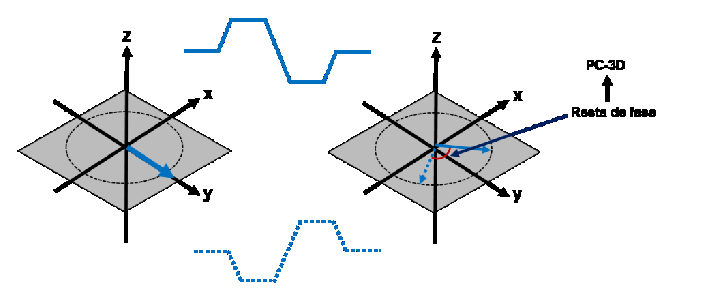
\includegraphics[width=\textwidth]{fig_arm_image17}
 \caption{
Método de procesamiento en ARM-PC. Para obtener la imagen se realiza una resta de fase es aquella donde se produce la resta de los cambios de fase que presentan los espines durante el cambio de gradiente y que son utilizadas para métodos de cortes delgados en PC-3D.
 }
 \label{fig:arm_image17}
\end{figg}
\end{figure}



\section{Angiografía con incremento de contraste por agentes exógenos}
La técnica de ARM con incremento de contraste ``Contrast-Enchanced'' (ARM-CE) fue descrita en el año de 1993, su principio es similar al de la angiografía convencional. En la ARM-CE se realiza la administración intravenosa de un bolo de agente de contraste extracelular derivado del gadolinio (Gd) antes o durante la adquisición de las imágenes. El Gd se ha utilizado en angiografía con técnicas TOF y CF con el objetivo de mejorar la relación señal-ruido y la visualización de pequeños vasos sanguíneos. El Gd es una tierra rara paramagnético (susceptibilidad magnética positiva) que favorece la relajación de los espines de su alrededor por lo que disminuye principalmente los tiempos \Tone que los de \Ttwo. 

El Gd es de elevada toxicidad pero unido a agentes quelantes, esta se ve disminuida, teniendo una gran seguridad para el uso en medicina diagnóstica. Las moléculas quelantes más utilizadas son la DTPA-BMEA (Optimark), DTPA (Magnevist), HP-DO3A (ProHance), DTPA-BMA (Omniscan), BOPTA (MutiHance) y DOTA (Dotarem). El Gd-DTPA tiene menos probabilidad de inducir reacciones adversas y son menos nefrotóxicos que los contrastes yodados, por lo que pueden utilizarse en pacientes con insuficiencia renal o en pacientes con transplantes de riñón (Figura \ref{fig:arm_image18}). 


El Gd-DTPA produce cambios en la susceptibilidad magnética de los tejidos, fundamentalmente provoca un acortamiento en los tiempos de relajación longitudinal modificando el \Tone de la sangre (rápida recuperación del vector de magnetización longitudinal) que no se satura aunque se usen TR muy cortos, mientras que los tejidos estacionarios sufren el efecto de la saturación y la consiguiente pérdida de señal. Dependiendo de la concentración de Gd-DTPA el valor \Tone de la sangre arterial puede ser disminuido de 50 a 100 ms. De esta forma se va aumentando la señal de la luz vascular (arterial y luego venosa) que se vuelve hiperintensa en secuencias potenciadas en \Tone. Posteriormente, el Gd, alcanza la circulación capilar y pasa al espacio intersticial, provocando un aumento de intensidad de los tejidos vascularizados, finalmente el Gd es ``lavado'' de los tejidos y eliminado por filtración glomerular. 


Siguiendo la inyección del bolo de agente de contraste, se observa el importante incremento local en la señal de la sangre. La sincronización entre el tiempo que pasa tras la inyección del Gd junto con el inicio de la secuencia es crítico para obtener una imagen correcta, en especial se debe asegurar que el llenado de las líneas del centro del espacio k, el cual aporta el contraste de la imagen, debe de coincidir con el pico máximo de concentración Gd en los vasos sanguíneos que queremos estudiar, que es en donde el agente de contraste es más estable. El inicio precoz de la secuencia dará como resultado un artefacto en anillo denominado \textit{ringing}, donde las paredes de los vasos se visualizan hiperintensas pero no el interior del vaso sanguíneo. Por otra parte, si se inicia la secuencia con retardo se producirá una contaminación de sangre venosa (Figura \ref{fig:arm_image19}). 


\begin{figure}[htbp]
\begin{figg}
 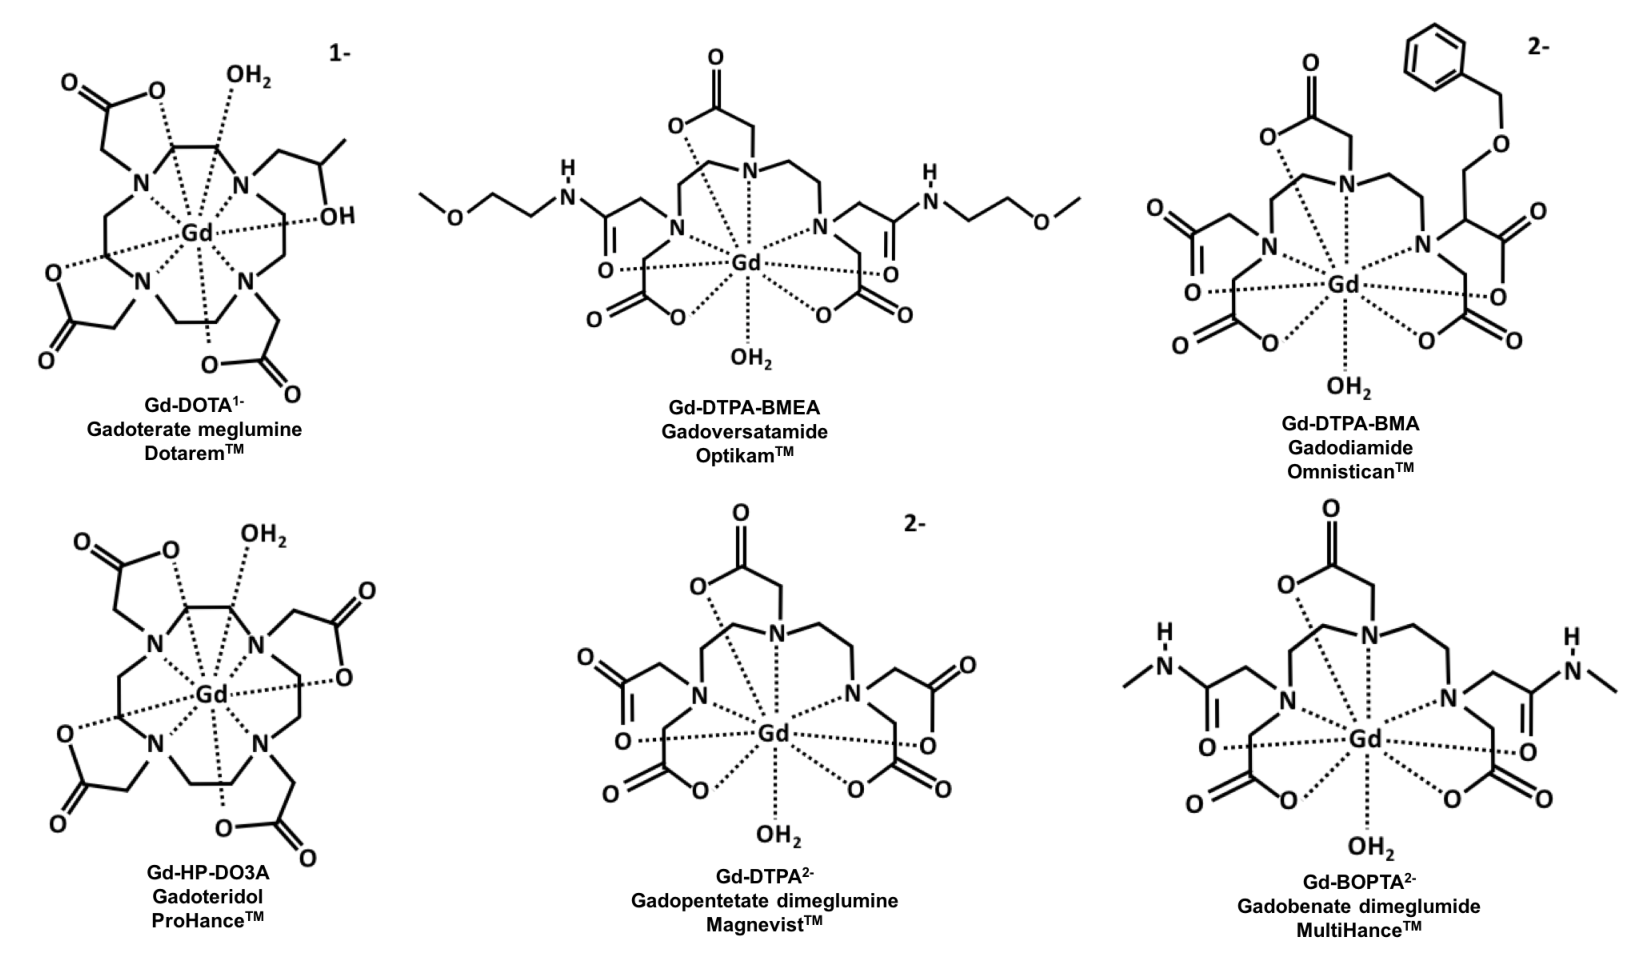
\includegraphics[width=\textwidth]{fig_arm_image18}
 \caption{
Quelatos de Gadolinio utilizados en CE-ARM. Se muestra la estructura química, nombre comercial y abreviatura de los quelatos que se han construido mediante química de coordinación. Se puede observar en todas las estructuras químicas como el Gd esta ``enjaulado'' dentro del quelato, asegurando así, la disminución de su toxicidad y resulte seguro utilizarlo en análisis de ARM..
 }
 \label{fig:arm_image18}
\end{figg}
\end{figure}


\begin{figure}[htbp]
\begin{figg}
 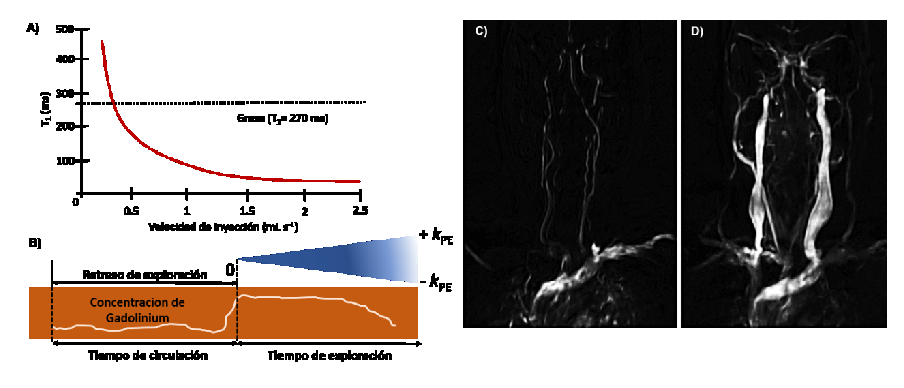
\includegraphics[width=\textwidth]{fig_arm_image19}
 \caption{
Efecto del incremento de contraste inducido por Gd. A) Efecto de reducción en valores \Tone en función de la velocidad de inyección de Gd-DTPA. Se muestra que el efecto del Gd sobre el tejido reduce su valor de \Tone mucho más que el de la grasa que generalmente es el más corto. B) Relación entre la concentración de Gd, el tiempo de circulación y la adquisición de datos para la codificación de fase del espacio K (KPE) en las imágenes 3D. C) Imagen con artefacto de ringing debido a inicio precoz de la secuencia. D) Imagen con contaminación venosa debido a inicio de la secuencia de forma tardía. 
 }
 \label{fig:arm_image19}
\end{figg}
\end{figure}



Para realizar estudios de ARM-CE intravenoso se emplean secuencias de adquisición EG en 3D con gradientes destructores de la magnetización remanente o equilibradas, que proporcionan una intensidad de señal proporcional a la concentración de Gd en la sangre. Este tipo de secuencias ultra-rápidas y la posibilidad de obtener imágenes de alta resolución espacial en 2D y 3D, permiten obtener un mayor realce del contraste en comparación con otras secuencias utilizando tiempos de adquisición relativamente cortos. Además, aumenta la sensibilidad para analizar la luz vascular, las estenosis y estudiar la perfusión de los tejidos sólidos (como el miocardio o ciertos tumores). 


En la Tabla \ref{tab:angio} se presenta la información más relevante sobre las ventajas y desventajas de cada una de las técnicas antes mencionadas. 



\section{Conclusión }
La ARM es una técnica diagnóstica ampliamente utilizada para poder evaluar la anotomía vascular. Mediante modificaciones en los gradientes de campo, la aplicación de secuencias de pulsos específicas, la sincronización cardiaca y la inyección de agentes de contraste, la ARM ha proporcionado información muy valiosa para caracterización y visualización el tejido vascular basándose únicamente en propiedades del flujo sanguíneo. Diversas técnicas pueden ser utilizadas con el objetivo de obtener la mejor información del tejido vascular las cuales utilizan las características del mismo flujo sanguíneo (dinámicas y magnéticas) para obtener el contraste sanguíneo. Estas técnicas han permitido caracterizar y diferencial el flujo sanguíneo arterial del venoso así como la magnitud, sentido y velocidad del flujo. 


% Please add the following required packages to your document preamble:
% \usepackage{booktabs}
\begin{table}[p]
\centering
\caption{Resumen de las ventajas y desventajas de las técnicas utilizadas en la ARM}
\label{tab:angio}
\begin{tabular}{l p{6cm} p{6cm}}
\toprule
\textbf{Técnica} & \textbf{Ventajas}                                                                                                                                                                                                                                           & \textbf{Desventajas}                                                                                                                                                                                                                                 \\ \midrule
\textbf{TOF-2D}  & Excelente contraste entre el tejido estacionario y el flujo sanguíneo. Mínimo efecto de saturación. Tiempos de adquisición cortos.Permite la adquisición de grandes estructuras vasculares. Alta sensibilidad al flujo lento en tiempos de adquisición cortos. & Baja relación señal ruido.Baja sensibilidad al flujo en el plano.Uso de rebanadas delgadas. Uso de valores TE largos.Sensible a sustancias con valores T1 cortos. Sensible al desfase intravoxel.Intensidad en el plano donde pasa el flujo sanguíneo. \\
\textbf{TOF-3D}  & Alta relación señal ruido.Alta resolución espacial. Menor desfase intravoxel. Mayor resolución de contornos de vasos delgados. Permite obtener rebanadas delgadas. Utiliza valores de TE cortos.                                                                & Produce saturación de flujos sanguíneos lentos. Baja sensibilidad a flujos lentos. Baja supresión del tejido de fondo. Sensible a sustancias con valores T1 cortos.                                                                                     \\
\textbf{PC-2D}   & Utiliza cortos tiempos de adquisición. Es sensible a los cambios de la velocidad del flujo sanguíneo. Buena supresión del tejido de fondo. Presenta mínimo efecto de saturación. No presenta sensibilidad a sustancias con valores de T1 cortos.                & Simple proyección del grosor de la sección. Produce artefactos de sobrelapamiento de vasos sanguíneos. Requiere buena estabilidad del sistema.                                                                                                         \\
\textbf{PC-3D}   & Permite obtener rebanadas delgadas. Es cuantitativa respecto a la velocidad y dirección del flujo. Buena supresión del tejido de fondo. Resulta ser sensible a la variabilidad en la velocidad del flujo. No presenta sensibilidad a cortas especies T1.        & Requiere tiempos de adquisición largos. Requiere valores de TE largos. No compensa la totalidad de la velocidad del flujo sanguíneo inherente.                                                                                                          \\
\textbf{ARM-CE}  & No presenta afectos de saturación. Reduce el desfase intravoxel. Alta resolución espacial. Emplea tiempos de adquisición cortos.Buena supresión del tejido de fondo.                                                                                           & Alto coste de los quelatos de Gd. Prescinde de la sincronización con el tiempo de inyección del bolo de Gd.                                                                                                                                           \\ \bottomrule
\end{tabular}
\end{table}


% \bibliographystyle{unsrt}
% \bibliography{cap_angio}

% \bibliography{libroResonancia}

